\documentclass[thesis.tex]{subfiles}

\begin{document}

% ----------------------------------------------------------
\chapter{Methodology} \label{chap:methodology}
% ----------------------------------------------------------
% Present the method and system. Basically write everything you've done.
% ----------------------------------------------------------


% ----------------------------------------------------------
\section{Dataset} \label{sec:data_collection}
% ----------------------------------------------------------
% Present how you gathered the data and labels
% ----------------------------------------------------------
%TODO : add list of diseases from datasets (like stated in \ref{sec:colon_cancer})

The datasets used in our experiments are Kvasir Pillcam, Kvasir and Hyper-Kvasir. This section will demonstrate the main differences between the three datasets and explain how they can be found and used for fact checking. All three datasets are collected using endoscopic equipment at Vestre Viken Health Trust in Norway. The VV consists of 4 hospitals and provides health care for 470.000 people. One of the hospitals is Bærum Hospital, which has a large gastroenterology department from where the data is collected. 



\subsection{Open-source endoscopy datasets}
% ----------------------------------------------------------
% Present other datasets found online, and end with what they lack,
% and why we need kvasirV2, hyper-kvasir, etc
% ----------------------------------------------------------


\subsection{Augere Medical}
% ----------------------------------------------------------
% Write about augere medical and the tagging tool and export script used
% ----------------------------------------------------------
Write about augere medical and the tagging tool and export script used



\subsection{Kvasir PillCam} \label{sec:kvasir_pillcam}
The dataset we used in our experiments consist of endoscopic videos collected from Bærum Hospital. Unlike Kvasir and Hyper-Kvasir datasets we have made the Kvasir PillCam dataset for the purpose of this thesis. In total we have 44 videos which have gone through some re encoding to reduce the file sizes, and also because the original encoding is proprietary Sony technology. After that the videos are uploaded to Augere Medical \footnote{\url{https://augere.md/}} tagging tool. The data export from Bærum also contains some findings for each video (if there is any) and are extracted, converted to frame number and that helped us a great deal with tagging the videos. We also have Thomas de Lange to thank, because he helped us a lot with the medical aspect of the classification process. When all 44 videos have been precisely labeled the dataset is exported from Augeres tagging tool and split into folders for each class. The folders/classes are given in table \ref{table:kvasir_pillcam}. In total we have 44 000 labeled images in 8 classes. The sample distribution across the eight classes is skewed depending on how many findings there are in the videos. Some findings occur often and some very rarely. The dataset also contain one class for 'normal' images, which there is quite a bit more of than findings. 

Imbalanced dataset pose a challenge for predictive algorithms as most learning algorithms are based on the assumption of an equal number of samples for each class. This results in models that have poor predictive performance, especially for minority class or classes. This is a great problem because in many medical datasets the minority class is the most important and therefore more sensitive for classification errors.

In addition to labeling the images the dataset also contain a JSON format file which stores coordinates for where in the frame the finding is located. The Kvasir Pillcam dataset will be an open-source dataset available for others scientists, and will later be grown to include more PillCam videos, both labeled and unlabeled samples.

\begin{table}
  \centering
  \begin{tabular}{ |c|c| }
  	\hline
  	Class number & Class name \\
    \hline
    0 & normal \\ 
    1 & polyp \\ 
    2 & polyrus \\ 
    \hline
  \end{tabular}
  \caption{PillCam class names and corresponding class numbers.}
  \label{table:kvasir_pillcam}
\end{table}


\subsection{Kvasir-V2} \label{sec:kvasir-v2}
The Kvasir dataset \cite{KVASIRMultiClass17} contains images from inside the gastrointestinal (GI) tract. The samples are classified into three important anatomical landmarks and three clinically significant findings. In addition it has two classes related to the removal procedure of polyps. The dataset is sorted and annotated is performed by medical doctors. The class names and findings for each class is given in table \ref{table:kvasir}. One of the most important aspects of the Kvasir dataset is that it makes it easy to reproduce and compare results in scientific computing.

\begin{table}
  \centering
  \begin{tabular}{ |c|c|c| }
  	\hline
  	Class number & Class name & Number of samples \\
    \hline
    0 & normal & 8000 \\ 
    1 & polyp & 8000 \\ 
    2 & polyrus & 8000 \\ 
    \hline
  \end{tabular}
  \caption{Kvasir class names and corresponding class numbers.}
  \label{table:kvasir}
\end{table}


\subsection{Hyper Kvasir} \label{sec:hyper_kvasir}
The Hyper-Kvasir dataset \cite{HyperKvasirComprehensive19} is one of the largest medical datasets containing 110.079 images and 373 videos where it captures anatomical landmarks and pathological and normal findings. Resulting in more than 1.1 million images and video frames all together. The dataset contain four parts, labeled images, unlabeled images, segmented images and lastly, videos. In total the dataset is 70 GB in size, but can be downloaded and stored in parts from \url{https://datasets.simula.no/hyper-kvasir/}.


\subsubsection{Labeled images}
Hyper-Kvasir contains 10.662 labeled images. The images are split into 23 different classes, and are stored in a folder with the same name as its corresponding class. All of the images are stored in JPEG format \cite{JPEGStill92}, which means it has some image quality loss but quite insignificant compared to the reduction in file size. Like in situations most often encountered the classes has a different number of samples, this is a challenge in the medical field because some findings occur more often than others.

% ask Pål for the figure with class/sample distribution from original hyper-kvasir paper

\subsubsection{Unlabeled images}
This part of the dataset contains 99.417 images

\subsubsection{segmented images}
In figure \ref{fig:kvasir_seg_example} we can see an example of the segmented Kvasir images.

\begin{figure}[H] % kvasir_seg_example
  \begin{center}
    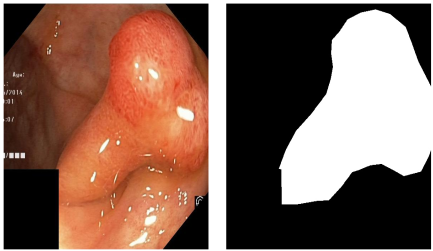
\includegraphics[width=0.7\textwidth]{kvasir_seg_example.png}
    \caption{Example of a segmented image from Hyper-Kvasir dataset.}
    \label{fig:kvasir_seg_example}
  \end{center}
\end{figure}


\subsubsection{Videos}




% ----------------------------------------------------------
\section{Data process} \label{sec:data_pipeline}
% ----------------------------------------------------------
% Present everything related to working with data files
% ----------------------------------------------------------

\subsection{Data preprocessing}
% data normalization, splitting, augmentation etc

\subsection{Data pipeline}
% tensorflow.data.Dataset pipeline with prefech, batching, shuffling, caching etc


% ----------------------------------------------------------
\section{System implementation} \label{sec:system_implementation}
% ----------------------------------------------------------
% Present the system architecture, some results perhaps
% ----------------------------------------------------------

% ----------------------------------------------------------
\section{Summary} \label{sec:C3-summary}
% ----------------------------------------------------------
% Present a summary of the chapter
% ----------------------------------------------------------


\end{document}